\documentclass[a4paper]{article}
\linespread{1.6}
\usepackage{geometry}
\usepackage{setspace}
\usepackage{amsmath}
\usepackage{amssymb}
\usepackage{enumerate}
\usepackage{subfigure}
\usepackage{caption}
\usepackage{listings}
\captionsetup{font = scriptsize}
\usepackage[pdftex]{graphicx}
\geometry{left=1cm,right=1cm,top=2.5cm,bottom=2.5cm}

\begin{document}
\begin{spacing}{2.0}
\begin{flushleft}\begin{huge}CAP6610  Machine Learning   Homework 2\end{huge}\end{flushleft}
\begin{flushright}\begin{Large}Hudanyun Sheng\end{Large}\end{flushright}
The MATLAB code used in this report are attached at the end of the report.
\begin{enumerate}[(1)]
\item The mutual information with the classes is defined as:
$$I(X; Y) = \sum_x\sum_y p(x,y)log\displaystyle\frac{p(x,y)}{p(x)p(y)}$$
\begin{figure}[h]
\centering
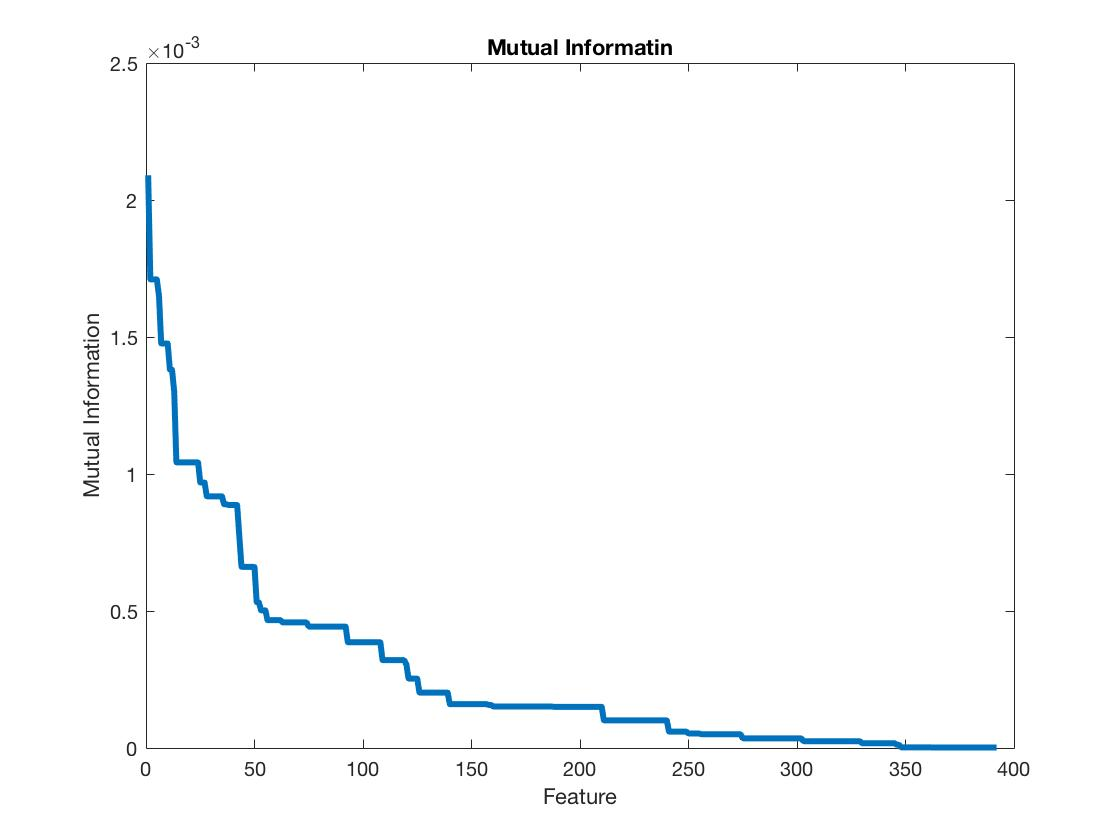
\includegraphics[width=3.5in]{MI.jpg}
\caption{Figure of sorted mutual information for each feature.}
\end{figure}

Based on the figure, we got to know that the first 120 features after sorting would be the most informative ones. The Naive Bayes Classifier built based on these features would get an error rate of 0.3386.

\item The generalization of the formula discussed in exercise 3.21 including multinomials is:
$$I_j = \sum_c\sum_j\theta_{jc}\pi_c log\displaystyle\frac{\theta_{jc}}{\theta_j}$$
where $\sum_c \pi_c = 1$

\item Suppose the true parameters for the prior Beta distribution are $a=b=20$, the prior distribution is shown below in figure \ref{beta1}. Now suppose we have the true prior distribution, i.e. the probability of 1 is 0.5, and the probability of 0 is also 0.5.\\ 
Now suppose the total number of experiments is 20, the posterior distribution looks like what shown in figure \ref{posterior1}. \\
Now keep the prior beta distribution to be the true one, and suppose the total number of experiments is 200, the posterior distribution is shown in figure \ref{posterior2}.\\
Keep the prior beta distribution to be the true one, and suppose the total number of experiments is 1000, the posterior

\begin{figure}[htbp]
\begin{minipage}[t]{0.5\linewidth}
\centering
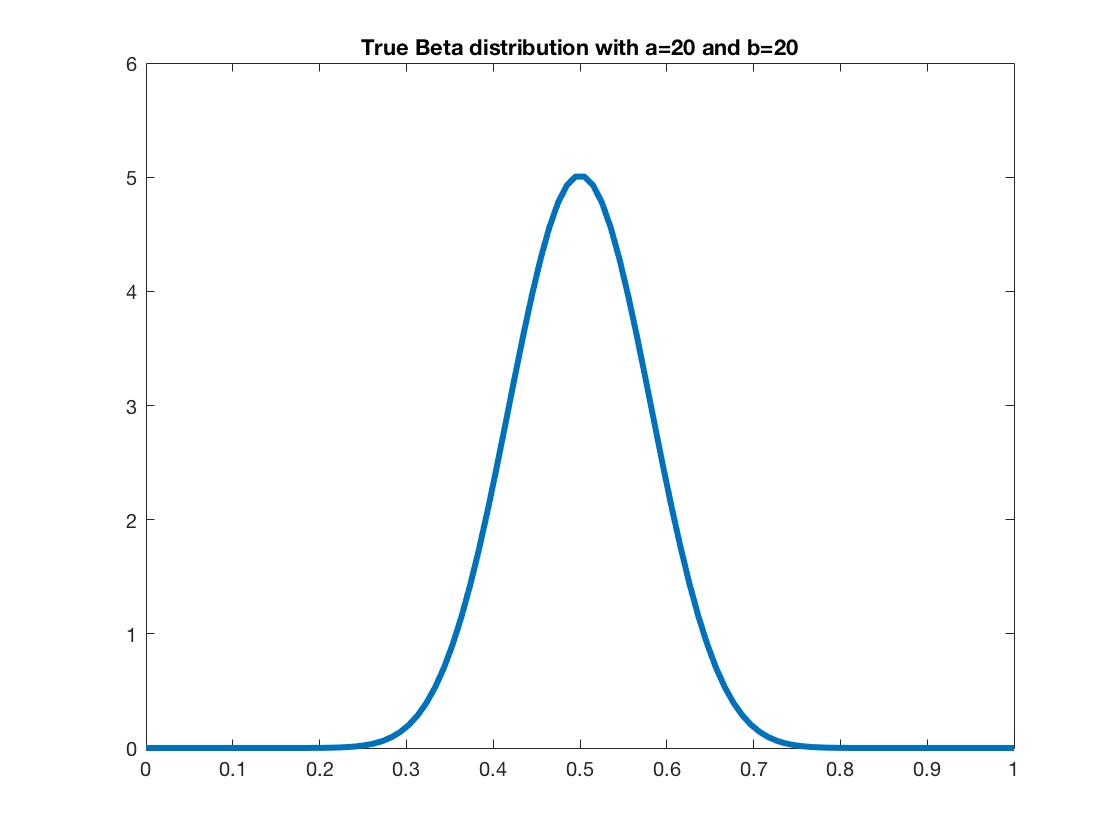
\includegraphics[width=3.4in]{Pbeta1.jpg}
\caption{Figure of the beta distribution with a=20 and b=20}
\label{beta1}
\end{minipage}
\begin{minipage}[t]{0.5\linewidth}
\centering
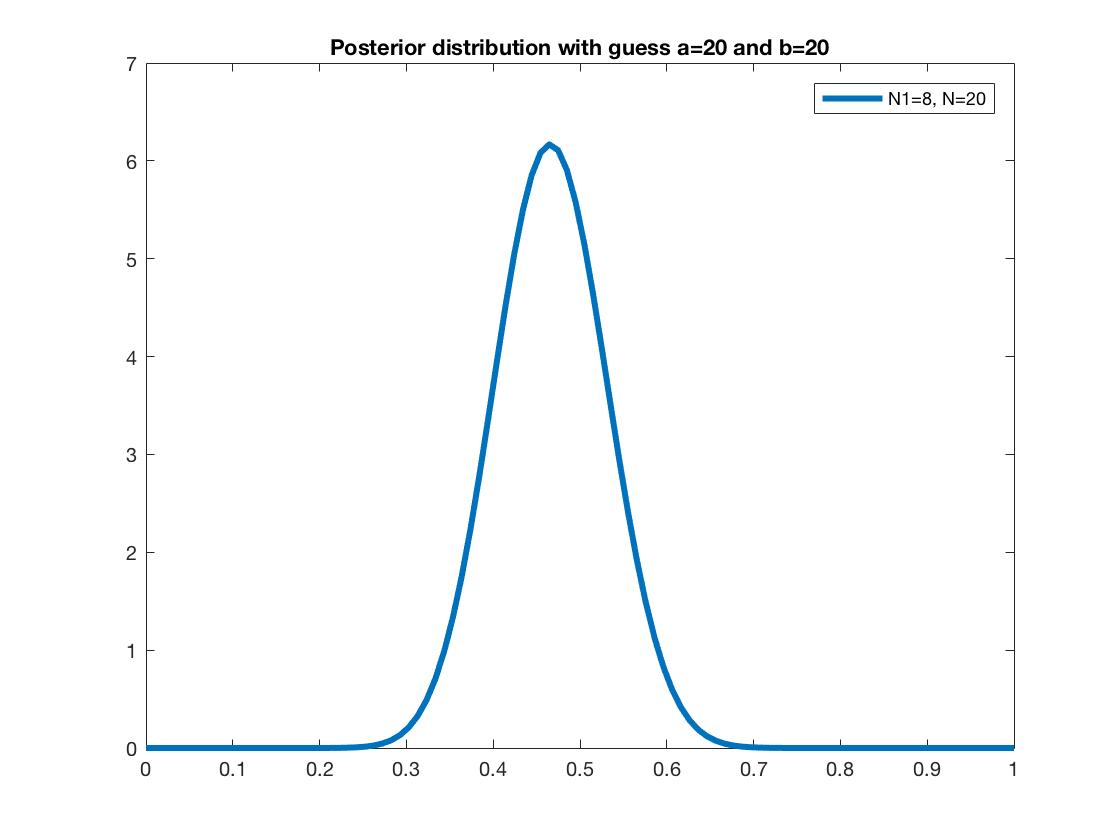
\includegraphics[width=3.4in]{posterior1.jpg}
\caption{Figure of the posterior distribution with a=20, b=20, N1=8, N=20}
\label{posterior1}
\end{minipage}
\end{figure}

\begin{figure}[htbp]
\begin{minipage}[t]{0.5\linewidth}
\centering
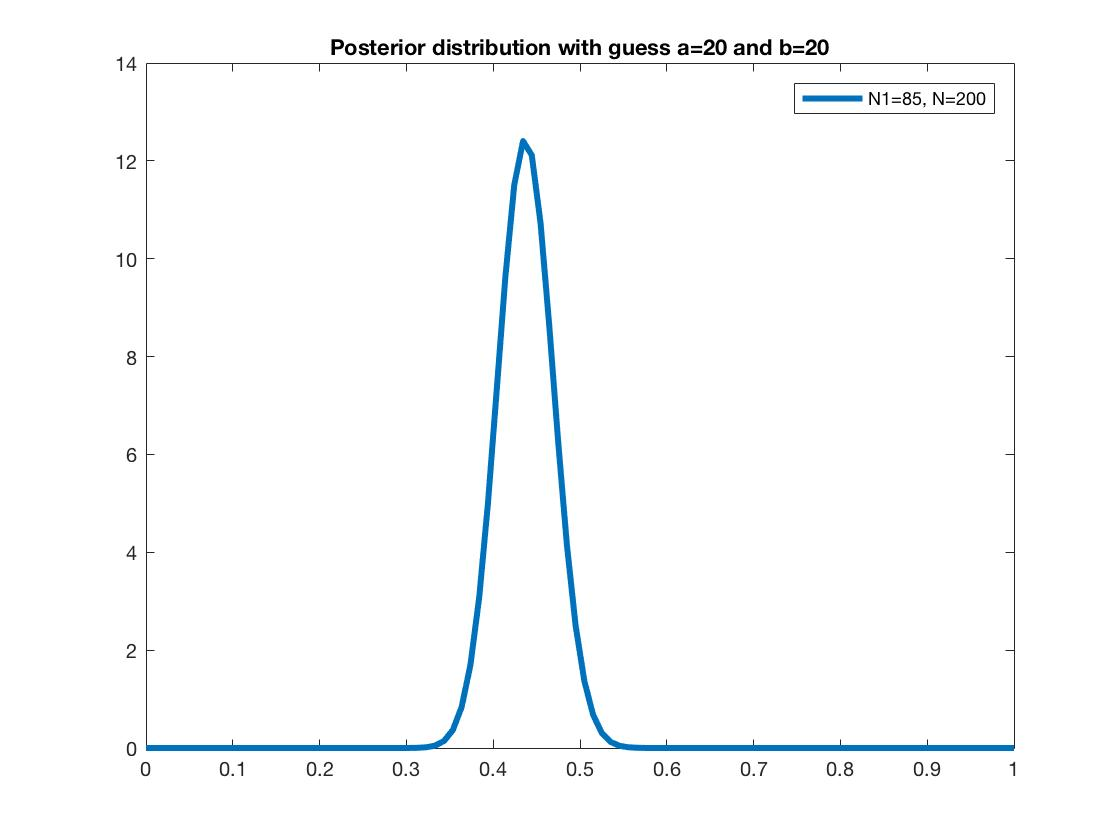
\includegraphics[width=3.4in]{posterior2.jpg}
\caption{Figure of the posterior distribution with a=20, b=20, N1=85, N=200}
\label{posterior2}
\end{minipage}
\begin{minipage}[t]{0.5\linewidth}
\centering
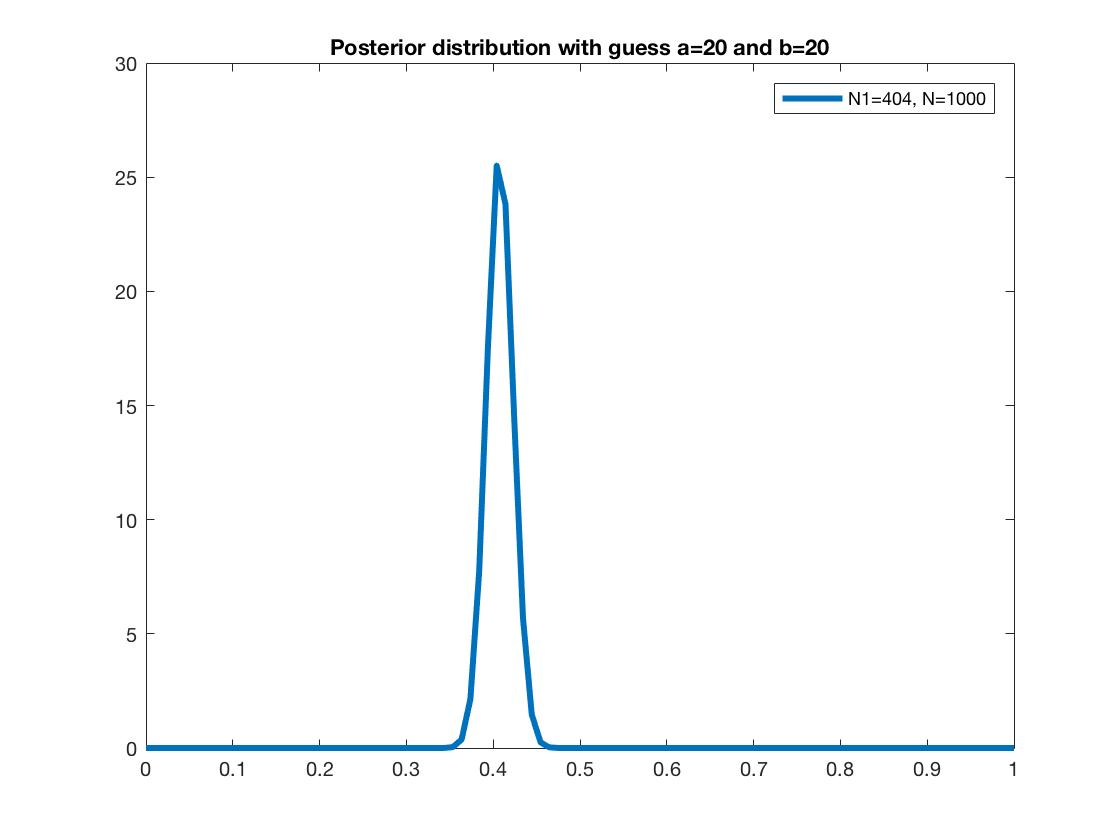
\includegraphics[width=3.4in]{posterior3.jpg}
\caption{Figure of the posterior distribution with a=20, b=20, N1=404, N=1000}
\label{posterior3}
\end{minipage}
\end{figure}

\begin{figure}[htbp]
\begin{minipage}[t]{0.5\linewidth}
\centering
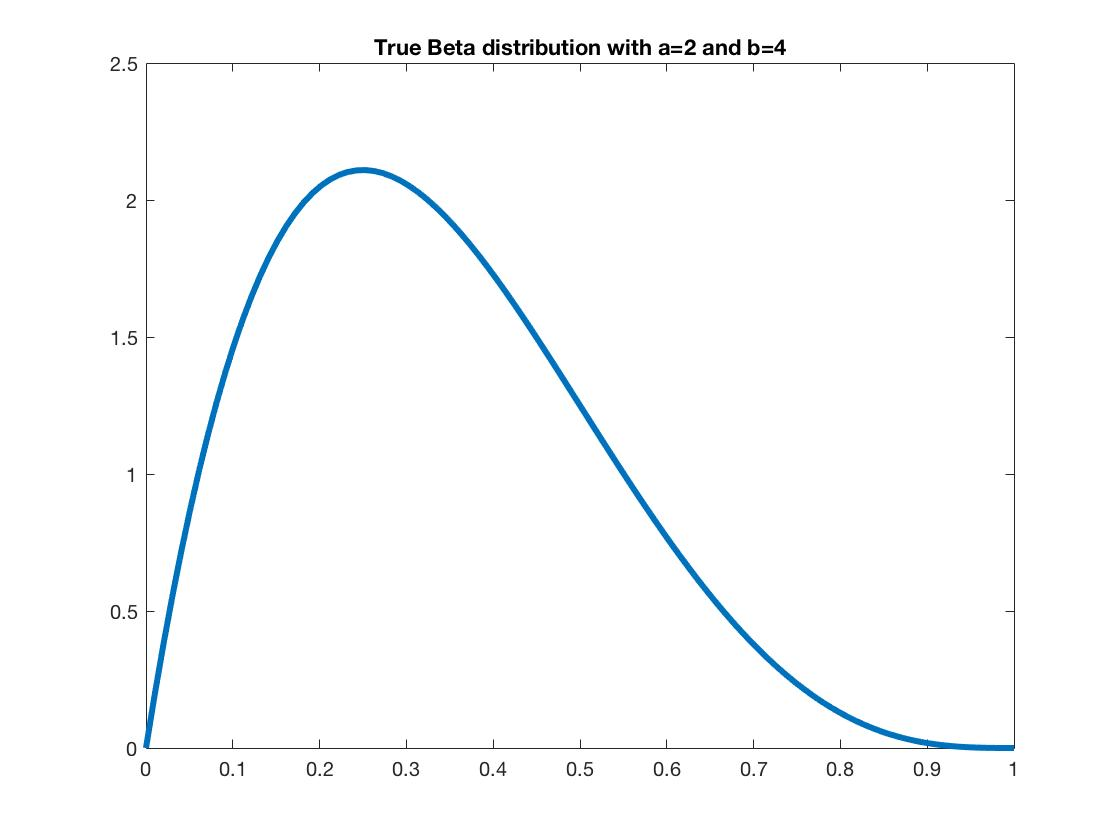
\includegraphics[width=3.4in]{Pbeta2.jpg}
\caption{Figure of the beta distribution with a=2 and b=4}
\label{beta2}
\end{minipage}
\begin{minipage}[t]{0.5\linewidth}
\centering
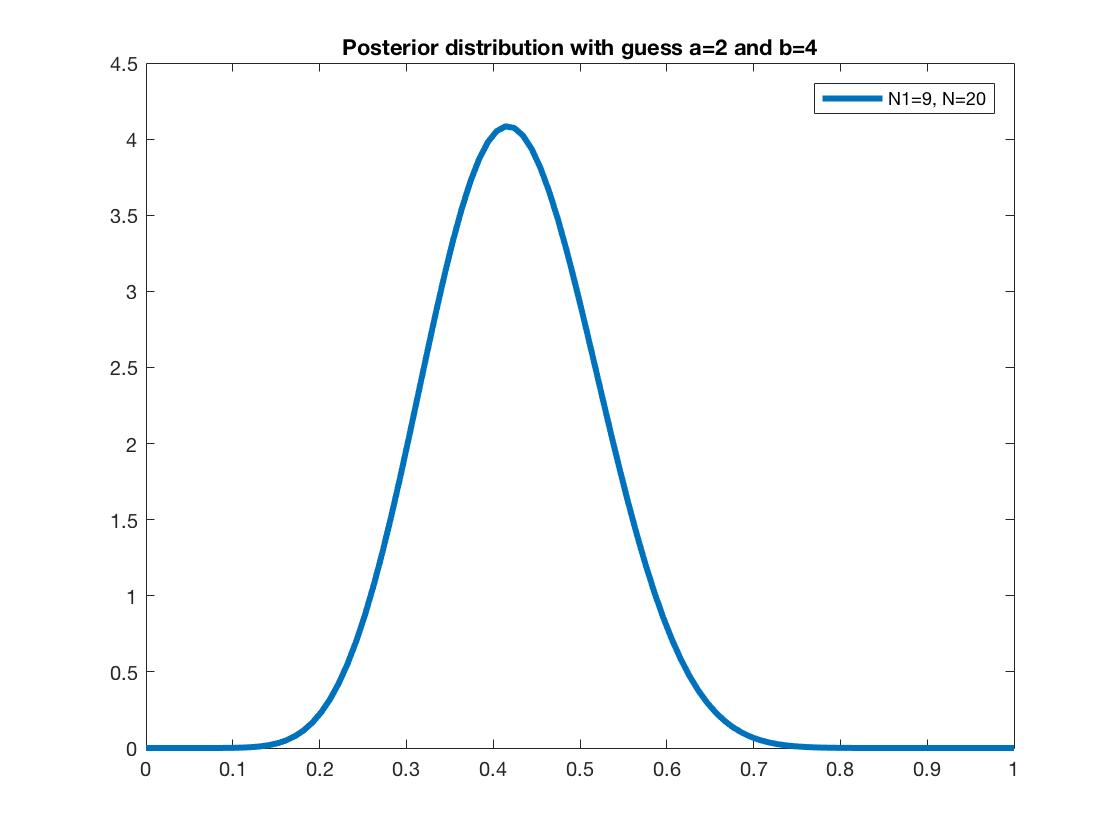
\includegraphics[width=3.4in]{posterior4.jpg}
\caption{Figure of the posterior distribution with a=2, b=4, N1=9, N=20}
\label{posterior4}
\end{minipage}
\end{figure}

\begin{figure}[htbp]
\begin{minipage}[t]{0.5\linewidth}
\centering
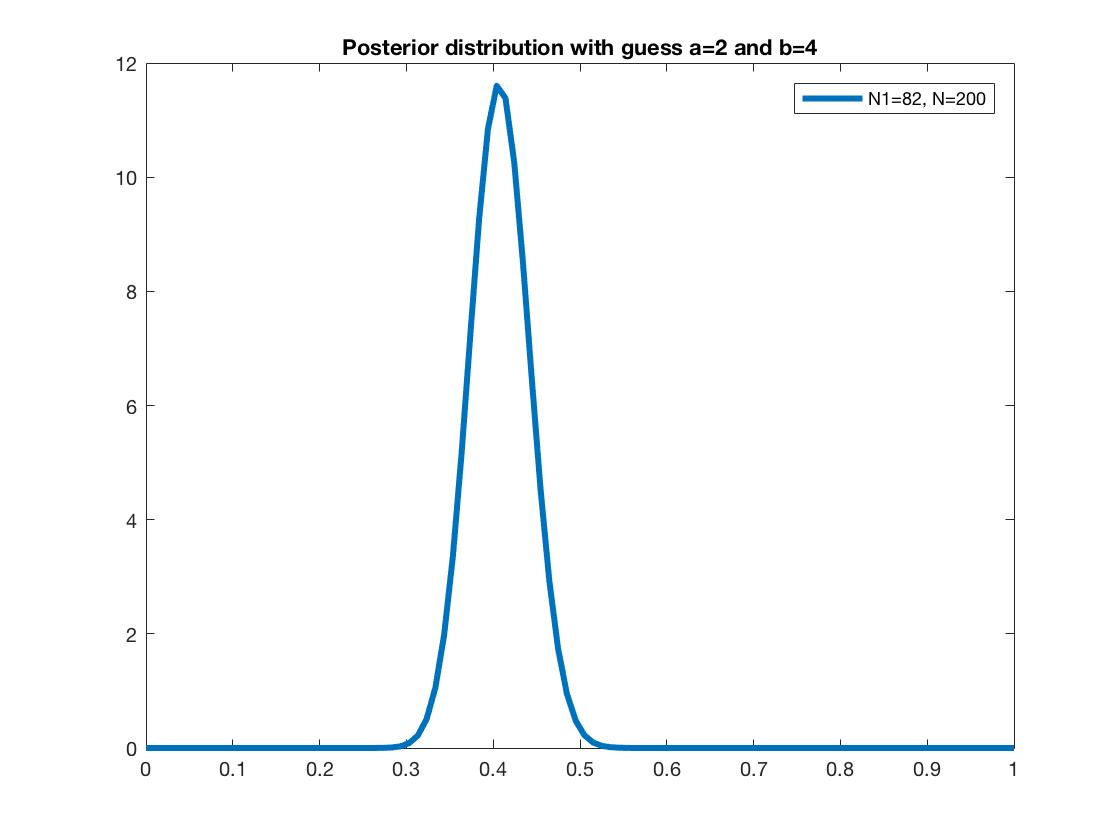
\includegraphics[width=3.4in]{posterior5.jpg}
\caption{Figure of the beta distribution with a=2, b=4, N1=82, N=200}
\label{posterior5}
\end{minipage}
\begin{minipage}[t]{0.5\linewidth}
\centering
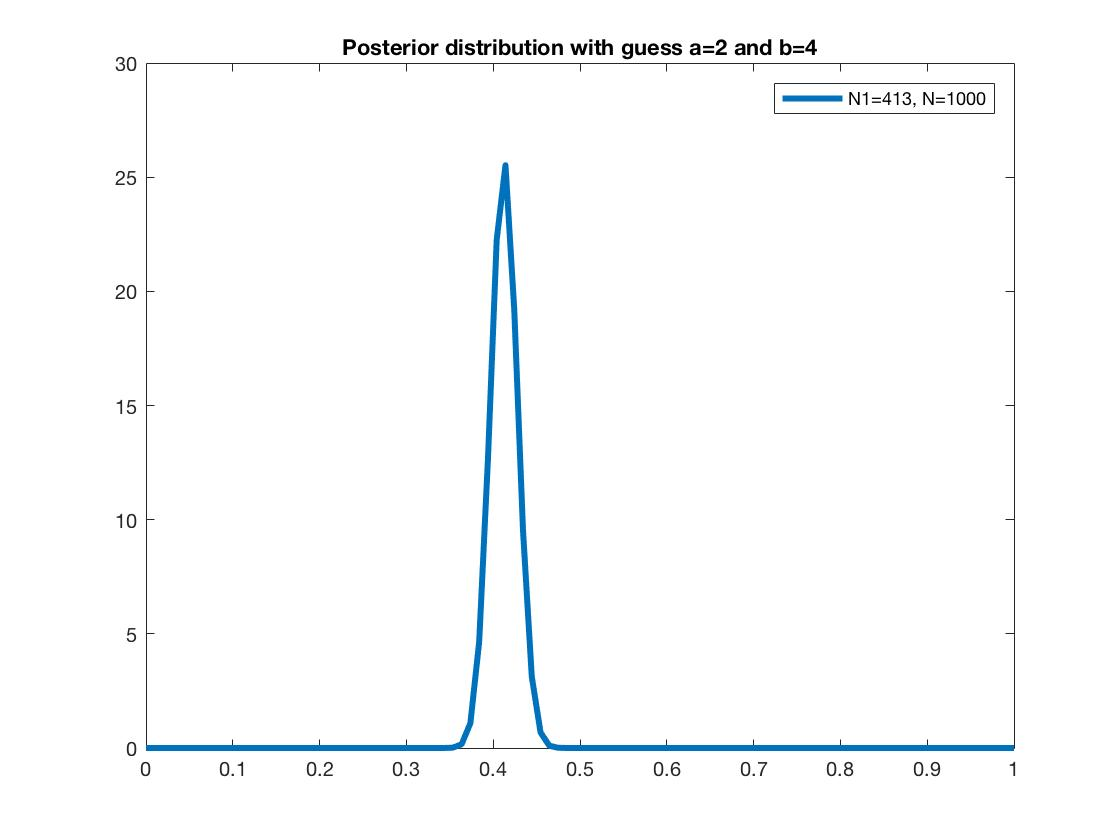
\includegraphics[width=3.4in]{posterior6.jpg}
\caption{Figure of the posterior distribution with a=2, b=4, N1=413, N=1000}
\label{posterior6}
\end{minipage}
\end{figure}


distribution is shown in figure \ref{posterior3}.\\
Now suppose we do not have the true prior distribution, but a prior beta distribution with a=2 and b=4. The distribution is shown in figure \ref{beta2}. Now suppose the total number of experiments is 20, the posterior distribution is shown in figure \ref{posterior4}.
Keep the prior beta distribution with a=2 and b=4, suppose the total number of experiments is 20, the posterior distribution is shown in figure \ref{posterior5}.\\
Keep the prior beta distribution, suppose the total  number of experiments is 2000, the posterior distribution is shown in figure \ref{posterior6}.\\
To conclude, when the number of samples is not enough, the prior would take over the posterior distribution,  but when the number of samples is large enough, the data would take over the posterior distribution.


\end{enumerate}


	
\end{spacing}
\end{document}